\documentclass[serif]{beamer}
\usepackage[english]{babel}
\usepackage[utf8]{inputenc}
% \usepackage[latin1]{inputenc}
\usepackage{graphicx}
\usetheme{Warsaw}
\usecolortheme{whale} %whale %beaver %seahorse
%\setbeamercolor{block body}{bg=white,fg=black}
%\setbeamercolor{block title}{bg=\usebeamercolor{frametitle},fg=black}	
\usepackage{amsmath}
\usepackage{psfrag}

\setbeamertemplate{headline}{}

\defbeamertemplate*{footline}{shadow theme}
{%
  \leavevmode%
  \hbox{\begin{beamercolorbox}[wd=.5\paperwidth,ht=2.5ex,dp=1.125ex,leftskip=.3cm plus1fil,rightskip=.3cm]{author in head/foot}%
    \usebeamerfont{author in head/foot} \insertshortauthor \hfill
  \end{beamercolorbox}%
  \begin{beamercolorbox}[wd=.5\paperwidth,ht=2.5ex,dp=1.125ex,leftskip=.3cm,rightskip=.3cm plus1fil]{title in head/foot}%
    \usebeamerfont{title in head/foot}\insertshorttitle \hfill \insertframenumber\,/\,\inserttotalframenumber%
  \end{beamercolorbox}}%
  \vskip0pt%
}

%\setbeamertemplate{headline}{%
%\leavevmode%
  %\hbox{%
    %\begin{beamercolorbox}[wd=\paperwidth,ht=3ex,dp=2ex]{author in head/foot}%
    %\hspace{1cm} \insertsection
    %\end{beamercolorbox}%
  %}
%}

\title[XFEM Stokes]{An Extended Finite Element Method for a Two-Phase Stokes problem}
\author[P. Lederer, C. Wintersteiger, C. Pfeiler]{P. Lederer, C. Wintersteiger, C. Pfeiler}
\institute[TU Wien]{TU Wien}
\date[25.6.2015]{25.6.2015}
\titlegraphic{
\includegraphics[width=1.5cm]{TU.eps}}


\begin{document}

\maketitle

\tableofcontents

%\begin{frame}{Inhaltsverzeichnis}
%\begin{itemize}
%\item Modellierung von chemischen Reaktionen
%\begin{itemize}
%\item Grundannahmen
%\item Herleitung
%\item Ordnungen
%\end{itemize}
%\item Differentialgleichungen + Numerik
%\item Allgemeine Geschichte von Schwingreaktionen
%\item Oszillierende chemische Reaktionen
%\item Numerische Ergebnisse
%\end{itemize}
%\end{frame}
%
\section{Physical problem}
\begin{frame}
  \frametitle{Physical problem}
  \begin{block}{} 
    problem ....
  \end{block}
\end{frame}

\subsection{Curvature}
\begin{frame}
  \frametitle{Curvature}

\end{frame}

\subsection{Bubble}
\begin{frame}
  \frametitle{Bubble}

\end{frame}

\subsection{Weak formulation}
\begin{frame}
  \frametitle{Weak formulation}

\end{frame}


\section{Discretization}

\begin{frame}
  \frametitle{Taylor Hood}
  \begin{block}{}
    ....
  \end{block}
\end{frame}


\subsection{LBB stability}
\begin{frame}
  \frametitle{LBB stability}
  \begin{block}{}
    ....
  \end{block}
\end{frame}


\subsection{Discontinuous pressure}
\begin{frame}
  \frametitle{Example with $f \neq 0$}
  \begin{block}{}
    ....
  \end{block}
\end{frame}

\section{Pressure enrichment}

\subsection{Discontinuous pessure}
\begin{frame}
  \frametitle{Example ... }
  \begin{block}{}
  \end{block}
\end{frame}

\subsection{Ghost penalty}
\begin{frame}
  \frametitle{Ghost penalty}
  \begin{block}{}
  \end{block}
\end{frame}

\begin{frame}
  \frametitle{Result with ghost penalty}
  \centering
  \begin{figure}
    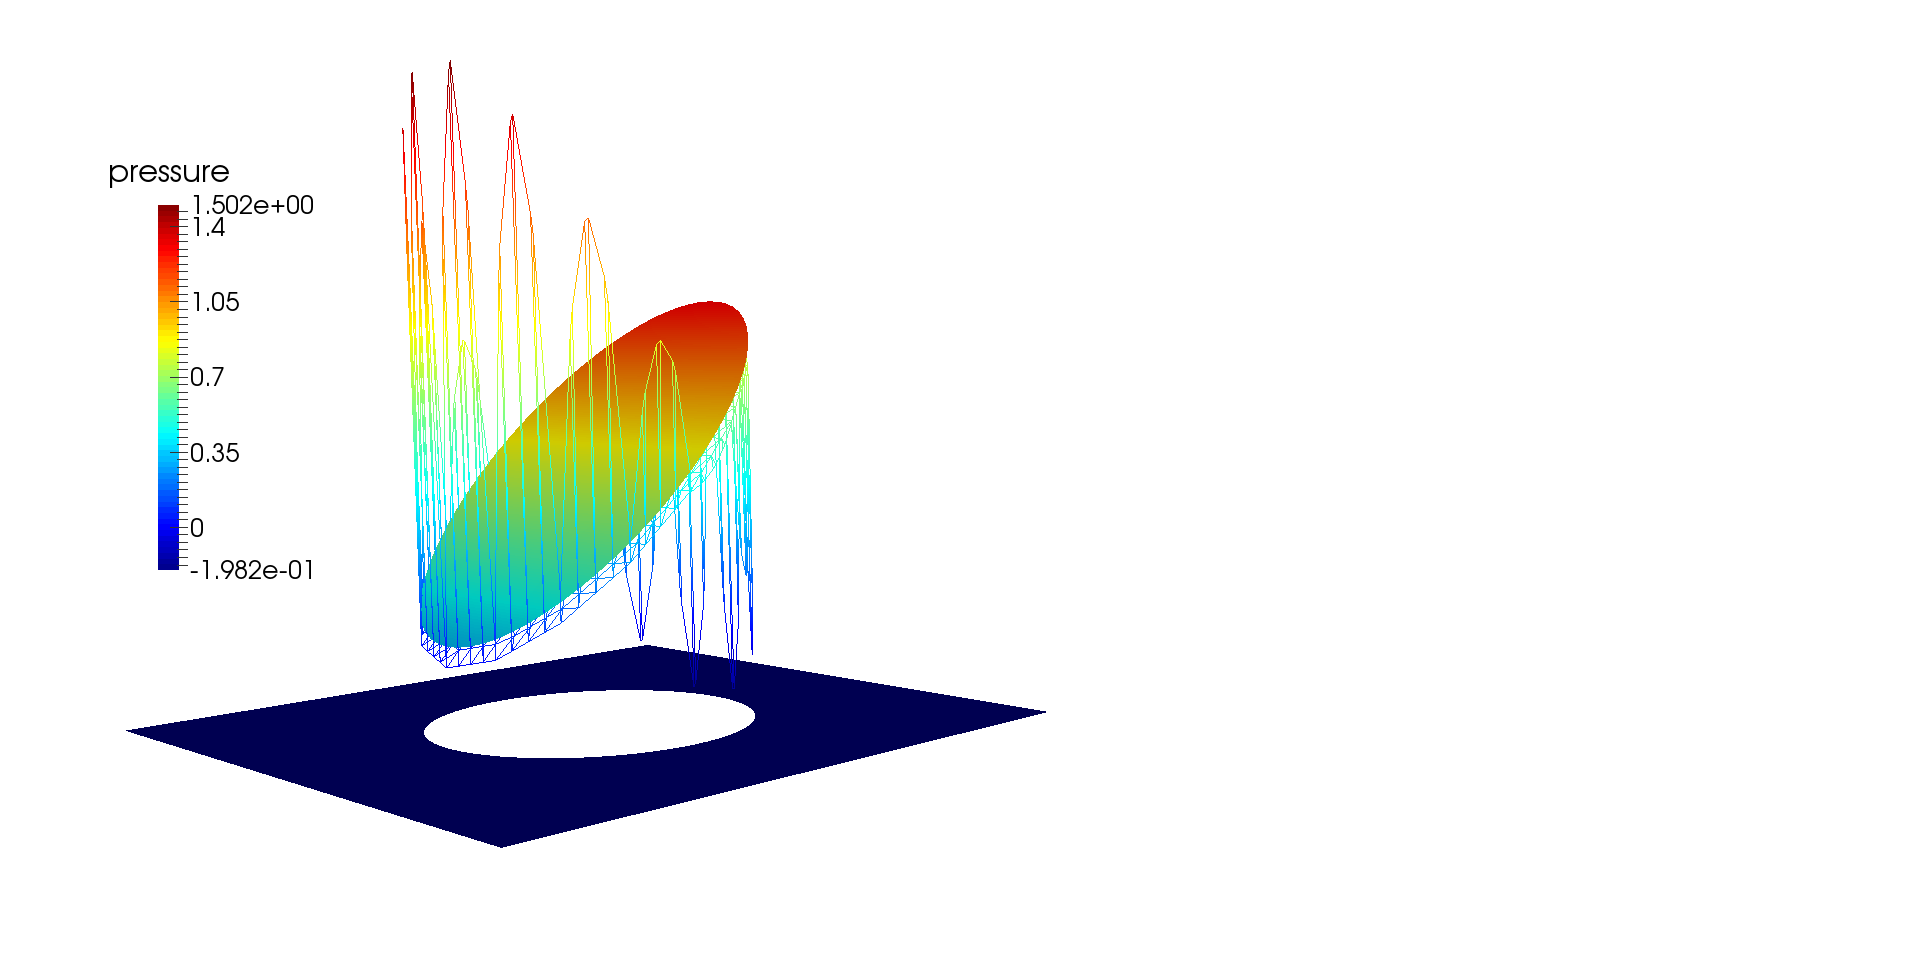
\includegraphics[height=0.5\paperheight, trim = 3cm 3cm 30cm 2cm , clip=true]{plots/together.png}
  \end{figure}
\end{frame}

%\begin{frame}
%\frametitle{Numerische Ergebnisse}
%\centering
%\vspace{-0.7cm}
%	\begin{figure}%
%		\hspace*{-0.4cm}
%		\subfloat{\includegraphics[width=0.3\paperwidth, trim = 1cm 6cm 2cm 6.5cm , clip=true]{zhab_HBrO2}}% [Bromige S�ure $\mathrm{HBrO_2}$]
%		\subfloat{\includegraphics[width=0.3\paperwidth, trim = 1cm 6cm 2cm 6.5cm , clip=true]{zhab_Br}}% [Brom $\mathrm{Br^-}$]
%		\subfloat{\includegraphics[width=0.3\paperwidth, trim = 1cm 6cm 2cm 6.5cm , clip=true]{zhab_H2O}}% [Wasser $\mathrm{H_2O}$]
%	\end{figure}%
%	\vspace{-1cm}
%	\begin{figure}%
%		\hspace*{-0.4cm}
%		\subfloat{\includegraphics[width=0.3\paperwidth, trim = 1cm 6cm 2cm 6.5cm , clip=true]{zhab_BrO3}}% [Bromat $\mathrm{BrO_3^-}$]
%		\subfloat{\includegraphics[width=0.3\paperwidth, trim = 1cm 6cm 2cm 6.5cm , clip=true]{zhab_HOBr}}% [Hypobromige S�ure $\mathrm{HBrO_2}$]
%		\visible<2->{\subfloat{\includegraphics[width=0.3\paperwidth, trim = 1cm 6cm 2cm 6.5cm , clip=true]{zhab_tau}}}% [Zeitschritt $\tau$]
%	\end{figure}
%\end{frame}
%
%\begin{frame}
%\frametitle{Grenzzyklus}
%Konzentrationen von bromiger S�ure $\mathrm{HBrO_2 = X}$, Brom $\mathrm{Br^-= Y}$ und Wasser $\mathrm{H_2O = Z}$ durchlaufen einen Grenzzyklus.
%\centering
%	\begin{figure}
%		\includegraphics[height=0.75\paperheight, trim = 0cm 0cm 0cm 2cm , clip=true]{orbit.ps}
%	\end{figure}
%\end{frame}

\section{Velocity enrichment}

\subsection{Kinks in velocity}

\begin{frame}
  \frametitle{Example $\mu_1 \neq \mu_2$ without enrichment}
  \begin{block}{}
  \end{block}
\end{frame}


\subsection{Nitsche}

\begin{frame}
  \frametitle{Nitsche}
  \begin{block}{}
    \begin{align}
      N(u,v) = ...
    \end{align}
  \end{block}
\end{frame}

\begin{frame}
  \frametitle{LBB stability?}
  \begin{block}{}
    ...
  \end{block}
\end{frame}


\section{Numerical example}


\begin{frame}
  \frametitle{Example $\mu_1 = \mu_2$}
  \begin{block}{}
  \end{block}
\end{frame}


\begin{frame}
  \frametitle{Example $\mu_1 \neq \mu_2$}
  \begin{block}{}
  \end{block}
\end{frame}

\end{document}
